% remember to set these at the start of each chapter
\chapter{CNN architectures} 
\label{cnn_architectures}
%%%%%%%%%%%%%%%%%%
In this section, three CNN architectures are discussed. A shallow five-layer CNN (Section \ref{arch_small}), a deeper 19-layer CNN VGG19 (Section \ref{arch_vgg}), and ResNet an advanced CNN with shortcut connections (Section \ref{arch_resnet}).

\section{Small CNN}
\label{arch_small}
This Small CNN architecrure is derived from \cite{Dhindsa2018}, which was used in grading the servery of prenatal hydronephrosis (PHN). This Small CNN has five convolutional layers, followed by a fully connected layer of 512 units and an output layer. Each layer (convolutional and fully connected) uses units with rectified linear (ReLU) activation functions. The output layer uses SoftMax activation function for classification. 

The first convolutional layer contains 16 filters with an input patch of $7 \times 7$ pixels. The second layer has 32 filters and an input patch size of $5 \times 5$ pixels. The following three convolutional layers contain 64 filters with patch size of 3 $\times$ 3 pixels. A stride is set to 1 in all convolutional layers. Padding is set to ‘same’, which results in padding the input such that the output has the same length as the original input.

Each convolutional layer is followed by a max pooling layer with 3 $\times$ 3 patch with a stride of 2 $\times$ 2 pixels. Pooling integrates the learned features in local patches and reduces the size of the image for subsequent layers. 

In addition to data augmentation, to reduce overfitting, batch normalization is performed after each convolutional layer, which normalizes the activations in a layer after a batch of images. Batch normalization subtracts the mean from the activations and divides the activations by the standard deviation. In order to make training more robust and efficient, dropout layer is added after the fully connected layer to reduce overfitting and to promote learning more independent features. At training phase, some nodes are dropped out with a dropout probability $p$. $p$ is set to 0.2.

\section{VGG}
\label{arch_vgg}

VGG is a CNN architecture that has significantly higher accuracy than prior models \citep{vgg}. It achieved state-of-the-art performance on the ILSVRC 2015 \citep{ILSVRC15} classification and localization tasks. 

\begin{figure}[h]
	\centering
	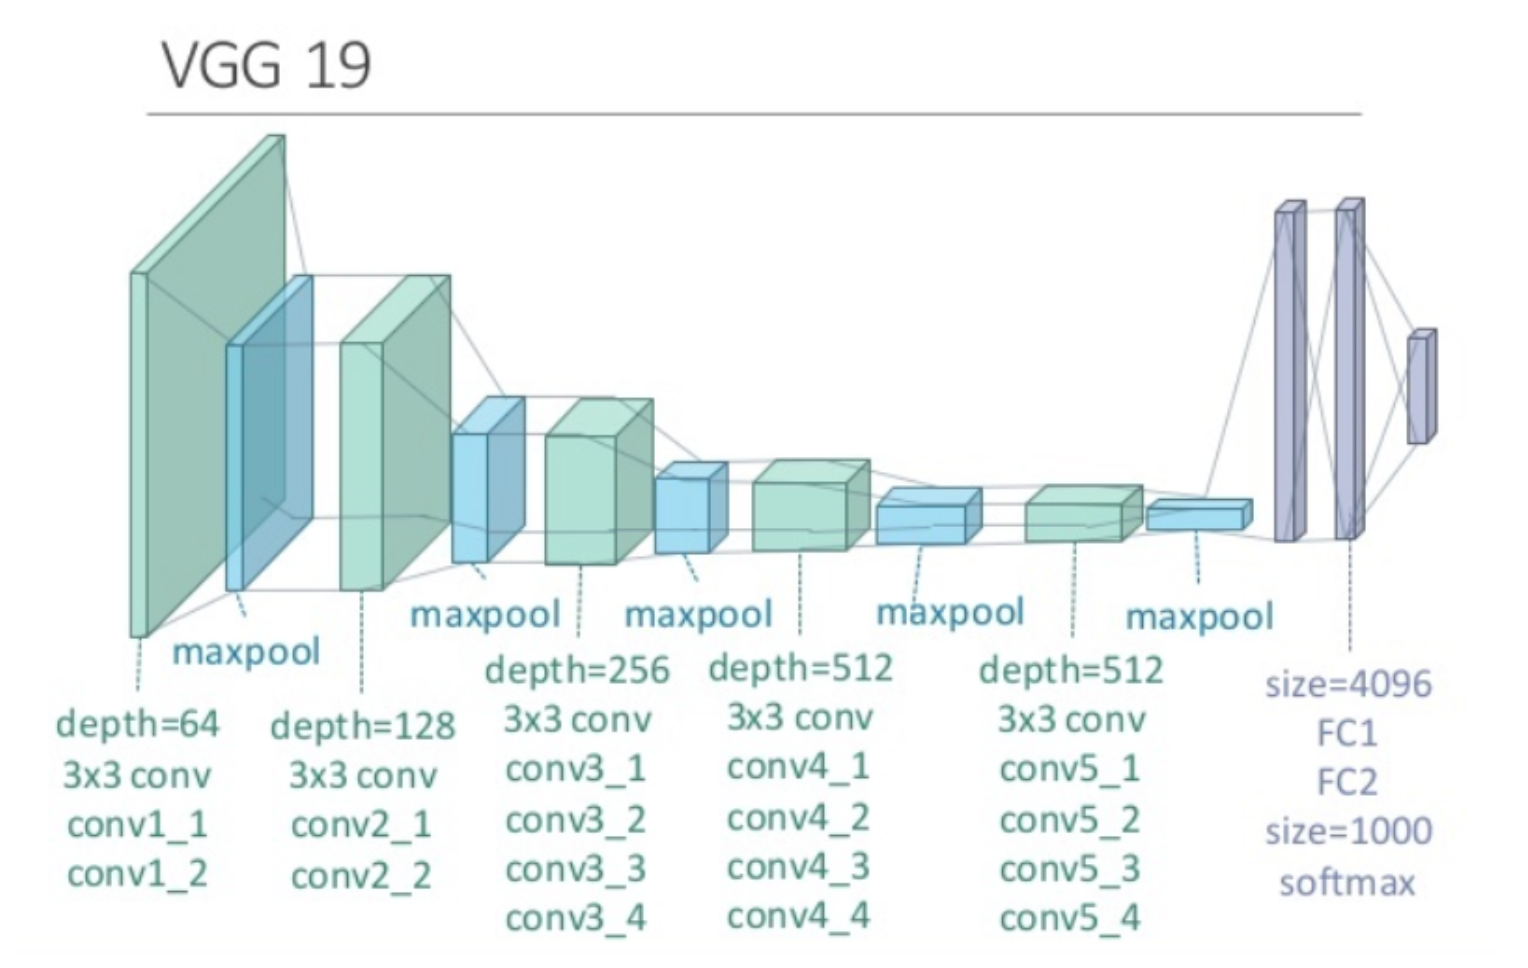
\includegraphics[scale=0.4]{Figs/vgg.png}
    \caption{VGG19 architecture \citep{Zheng2018}}
    \label{VGG}
\end{figure}

  Fig.\,\ref{VGG} shows a VGG19 architecture. The input image is passed through a stack of convolutional layers. The filter that is used has a very small receptive field: 3 $\times$ 3 (which is the smallest size to capture the notion of left/right, up/down, center). Padding is set to "same". The convolution stride is 1. A max-pooling layer is added after two convolution layers for the first two blocks. For the third, fourth and fifth block, the setup is four convolution layers then a max-pooling layer. All max-pooling is performed over a 2 $\times$ 2 pixel window, with stride 2 $\times$ 2 pixels. A stack of convolutional and max-pooling blocks is followed by three fully connected layers: the first two have 4096 channels each, the third performs classification. All hidden layers use the ReLU activation function. The final layer has Softmax activation function for classification. Dropout layers are added between two fully connected layers. Dropout rate is set to 0.5.

Rather than using relatively large receptive fields in the convolutional layers, VGG uses very small 3 $\times$ 3 receptive fields throughout the whole net. However, the receptive field of a stack of two 3 $\times$ 3 convolutional layers is the same as that of a 5 $\times$ 5 convolutional layer; three 3 $\times$ 3 layers has the effective receptive field as a 7 $\times$ 7 layer. 

Comparing to a single 7 $\times$ 7 convolution layer, a stack of three 3 $\times$ 3 convolution layers give the benefit of incorporating three non-linear rectification layers instead of a single one, which makes the decision function more discriminative. Also, the number of parameter is decreased. A stack of three 3 $\times$ 3 filters have $3\times3^2 = 27$ parameters whereas a 7 $\times$ 7 filter has $7^2 = 49$ parameters. 

To limit the number of free parameters and improve training efficiency, some trained weights from other dataset can be re-used. This strategy is Transfer Learning \citep{transfer}. VGG-IN is a VGG model with ImageNet \citep{imagenet_cvpr09} pre-trained weights \citep{vgg} loaded and locked in the convolutional layers, only fully connected layer and classification output layer are retrained to fit our problem.

\section{ResNet}
\label{arch_resnet}

The depth of a neural network is an important factor affecting performance. The architecture used in visual tasks is often very deep, such as VGG discussed above. We usually achieve better accuracy with deeper neural networks. However, when the network is too deep, we may encounter the vanishing gradient problem. In back propagation, a weight is updated proportional to the partial derivative of the error function with respect to the current weight, as derived in Sec.\,\ref{back-prob}. In some cases, the gradient will be vanishingly very small. This will prevent the weight from updating. In the worst case, this may completely stop the neural network from further training. When networks get deeper, a degradation problem rises. From \citeauthor{Srivastava2015}'s experiments \cite{Srivastava2015} (Fig.\,\ref{deeploss}), the more layers in a deep neural network model, the higher the training error is. Accuracy gets saturated sooner with the network depth increases.

\begin{figure}[h]
	\centering
	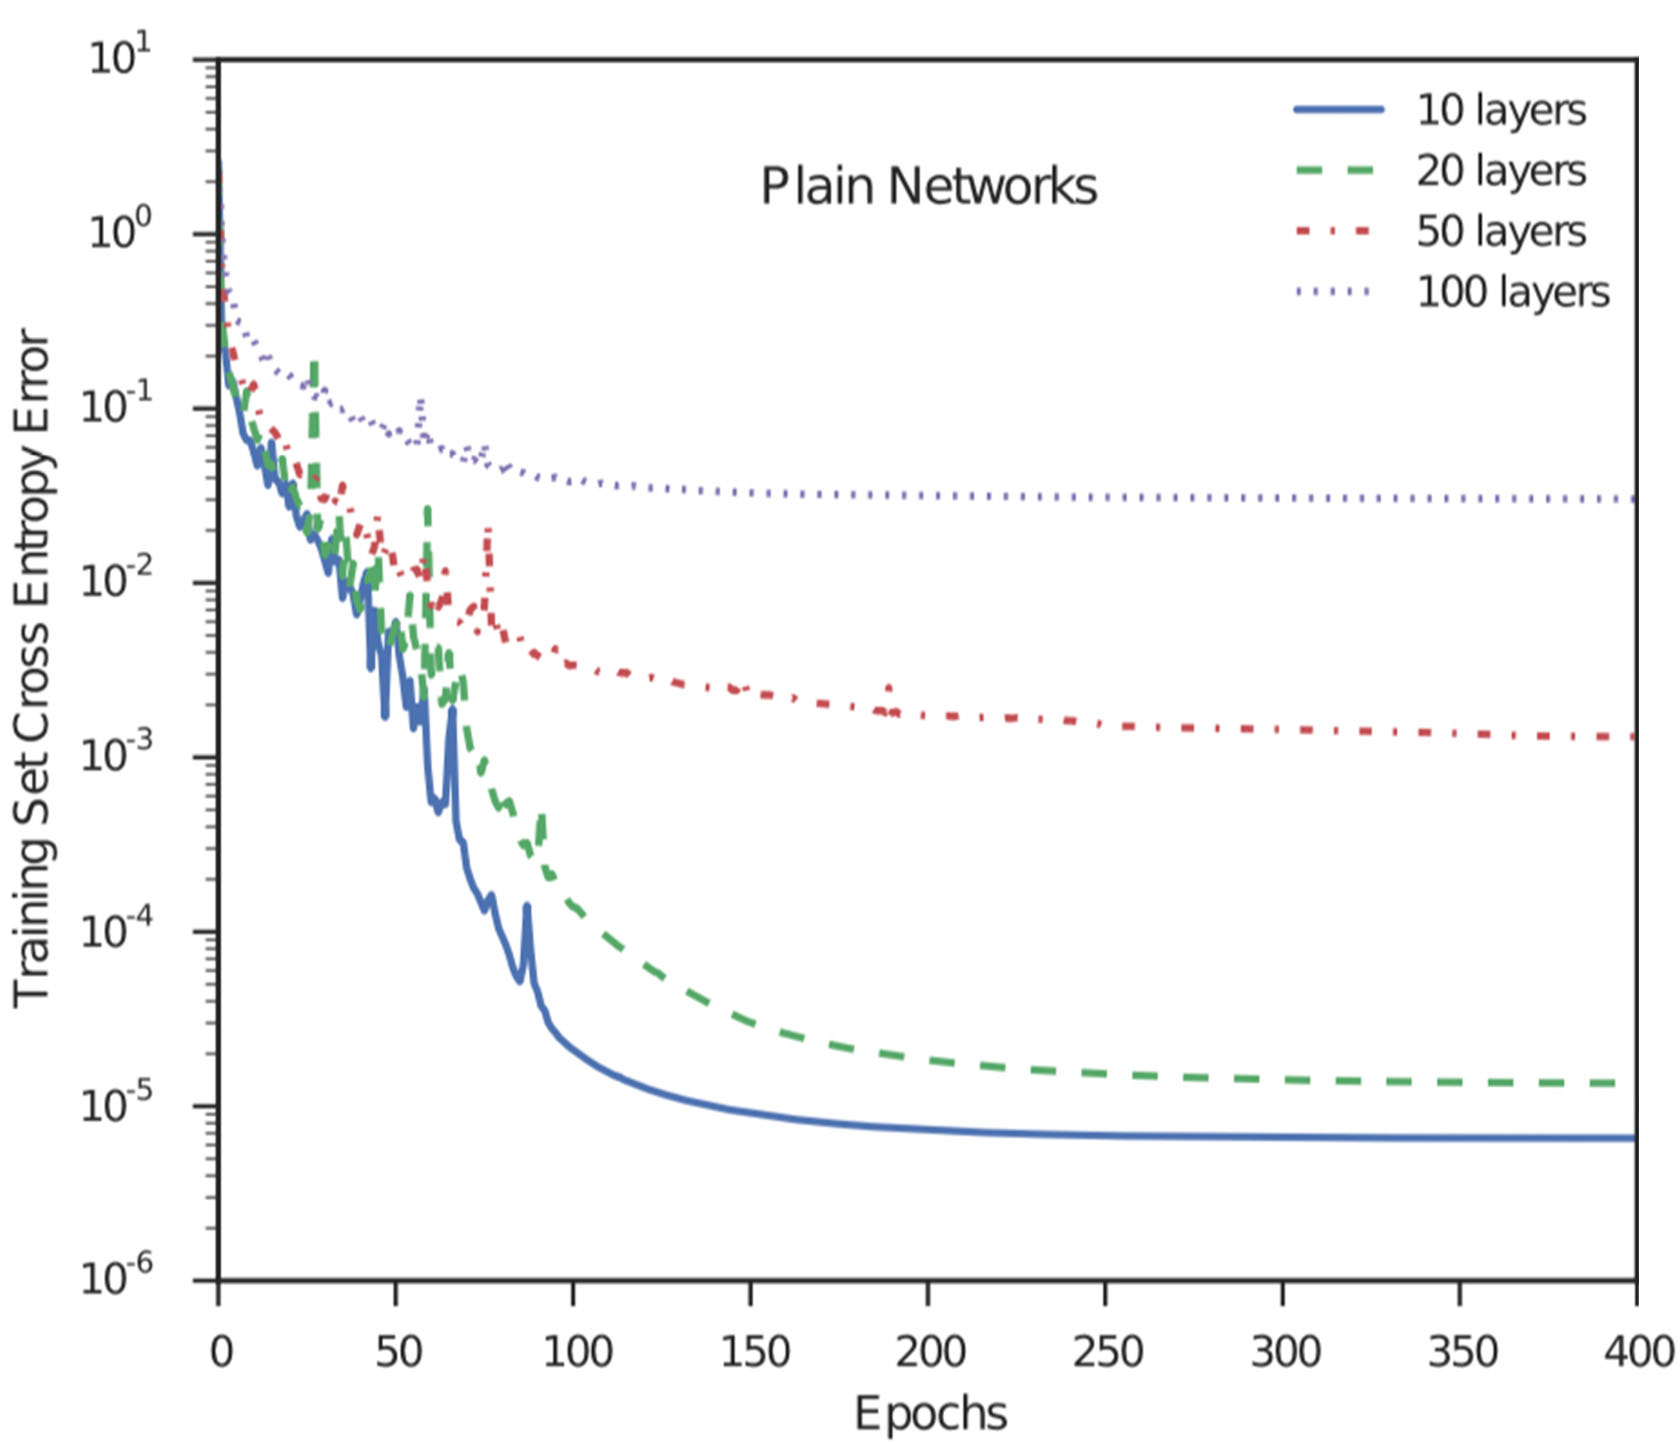
\includegraphics[scale=0.5]{Figs/deeploss.jpg}
    \caption{Training Loss: Deep vs. Shallow \cite{Srivastava2015}}
    \label{deeploss}
\end{figure}

The degradation problem is addressed by ResNet  \citep{resnet}. Intuitively, if we know a shallower network performs better than a deeper counterpart with few extra layers, we may skip the extra layers to achieve an accuracy that at least matches the shallower network. In ResNet, such skipping is done by shortcuts. Shortcuts provide residual connections straight to earlier layers. As seen in Fig.\,\ref{residualblock}, the residual connection directly adds the value at the beginning of the block, $\mathbf{x}$, to the end of the block $\mathcal{F}(\mathbf{x})+\mathbf{x}$. This residual connection does not go through activation function, thus the derivatives may not vanish and learning is less likely to stall. Shortcut connections simply perform identity mapping. They add neither extra parameter nor computational complexity. The entire network can still be trained with back propagation.

\begin{figure}[h]
	\centering
	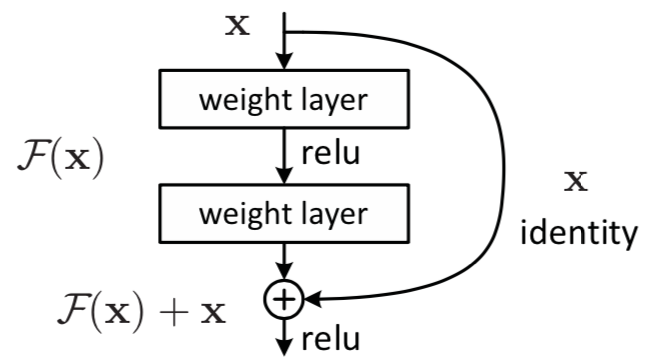
\includegraphics[scale=0.5]{Figs/residualblock.png}
    \caption{Residual learning: a building block \cite{resnet}}
    \label{residualblock}
\end{figure}


Residual learning:
A block of layers should approximate an underlying mapping from its input to output. Let $\mathcal{H}(\mathbf{x})$ denote this mapping. $\mathbf{x}$ denotes the input to the block. In a neural network, it is known that a stack of layers can learn a complex function to approximate the underlying mapping $\mathcal{H}(\mathbf{x})$. In ResNet, instead of the stacked layers to approximate $\mathcal{H}(\mathbf{x})$, let these layers approximate a residual function $\mathcal{F}(\mathbf{x}) := \mathcal{H}(\mathbf{x})-\mathbf{x}$. The original mapping thus becomes $\mathcal{F}(\mathbf{x})+\mathbf{x}$. 

A deeper neural network model should have training error no greater than its shallower counterpart if the extra layers can be constructed as identity mappings. In theory, a few stacked layers should be able to approximate any function including an identity mapping. However, the degradation problem suggests that the solvers might have difficulties in approximating identity mappings by multiple nonlinear layers. With the residual learning reformulation, if identity mappings are optimal, the solvers may simply drive the weights of the multiple nonlinear layers toward zero to approach identity mappings. 

Identity mapping by shortcuts: 
As shown in Fig.\,\ref{residualblock}, a few stacked layers are equipped with a residual connection, this is a building block of ResNet. Formally, a building block is defined as: 
\begin{equation} \label{eq1}
\mathbf{y} = \mathcal{F} (\mathbf{x}, \{W_i\}) + \mathbf{x}
\end{equation}

Here $\mathbf{x}$ and $\mathbf{y}$ are the input and output vectors of a block, $W$ denotes learnable weights. The function $\mathcal{F} (\mathbf{x}, \{W_i\})$ represents the residual mapping to be learned. For the example in Fig.\,\ref{residualblock} that has two layers, $\mathcal{F}=W_2\sigma(W_1\mathbf{X})$, $\sigma$ denotes ReLU activation function. The operation $\mathcal{F} + \mathbf{x}$ is performed by a shortcut connection and element-wise addition. A second ReLu activation $\sigma(\mathbf{y})$ is applied after the addition. The shortcut connection in (\ref{eq1}) introduces neither extra parameter nor computation complexity. The dimensions of $\mathbf{x}$ and $\mathcal{F}$ must be equal in (\ref{eq1}). When the input and output do not have equal dimensions, a linear projection $W_s$ is added to the shortcut connections (\ref{eq2}) to match the dimensions: 

\begin{equation} \label{eq2}
\mathbf{y} = \mathcal{F} (\mathbf{x}, \{W_i\}) + W_s \mathbf{x}
\end{equation}

$W_s$ is identity mapping and only used when matching dimensions. 

Although the above notations and equations only demonstrate fully-connected layers for simplicity, they are also applicable to convolutional layers. The function $\mathcal{F} (\mathbf{x}, \{W_i\})$ can represent multiple convolutional layers.

The following describes an implementation of ResNet18 \citep{resnet_implement}:

There are two types of ResNet block, depending on whether the input-output dimensions are same (\ref{eq1}) or different (\ref{eq2}). We call them Identity Block and Convolutional Block. CONV2D refers to 2D convolutional layer. BatchNorm refers to batch normalization.

\begin{figure}[h]
	\centering
	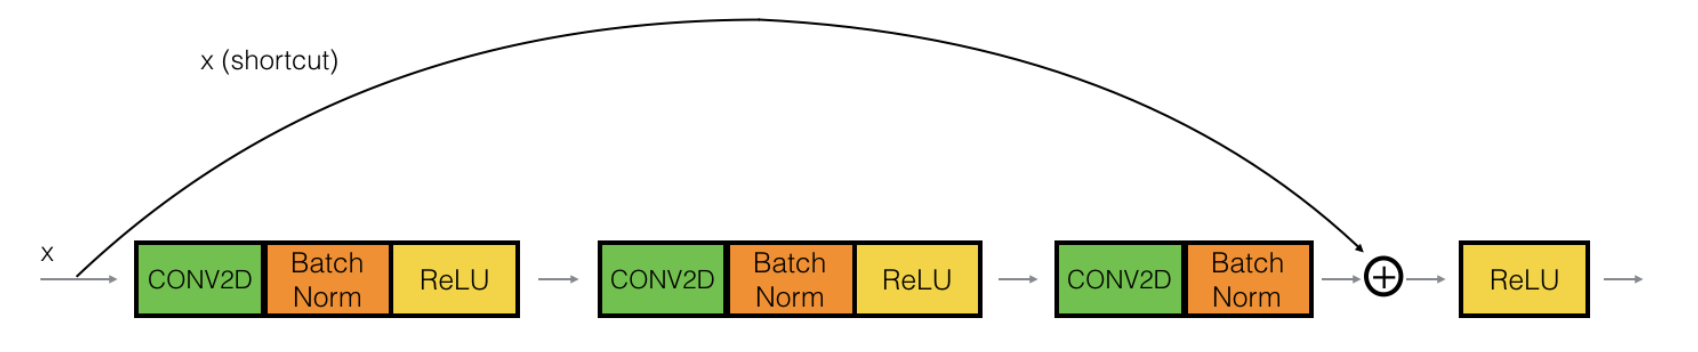
\includegraphics[width=\textwidth]{Figs/identityblock.png}
    \caption{Identity Block \citep{resnet_implement}}
    \label{identityblock}
\end{figure}

\begin{enumerate}
\item  Identity Block (Fig.\,\ref{identityblock}) is used in the case where the input of the block has the same dimension as the output, formally defined in (\ref{eq1}).
    \begin{description}
      \item[$\ast$ First component of main path:] The first CONV2D has $F_1$ filters of shape (1,1) and a stride of (1,1). Its padding is "valid", which means no padding. The first BatchNorm is normalizing the channels axis. Then apply the ReLU activation function. 
      \item[$\ast$ Second component of main path:] The second CONV2D has $F_2$ filters of shape $(f,f)$ and a stride of (1,1). Its padding is "same", meaning the output is padded to the same size of input. The second BatchNorm is normalizing the channels axis. Then apply the ReLU activation function. 
      \item[$\ast$ Third component of main path:] The third CONV2D has $F_3$ filters of shape (1,1) and a stride of (1,1). Its padding is "valid". The third BatchNorm is normalizing the channels axis. Note that there is no ReLU activation function in this component.
      \item[$\ast$ Shortcut path:] Shortcut path is just simply the input.
      \item[$\ast$ Final step:] The shortcut and the input are added together. Then apply the ReLU activation function.
    \end{description}
    
\begin{figure}[h]
\centering
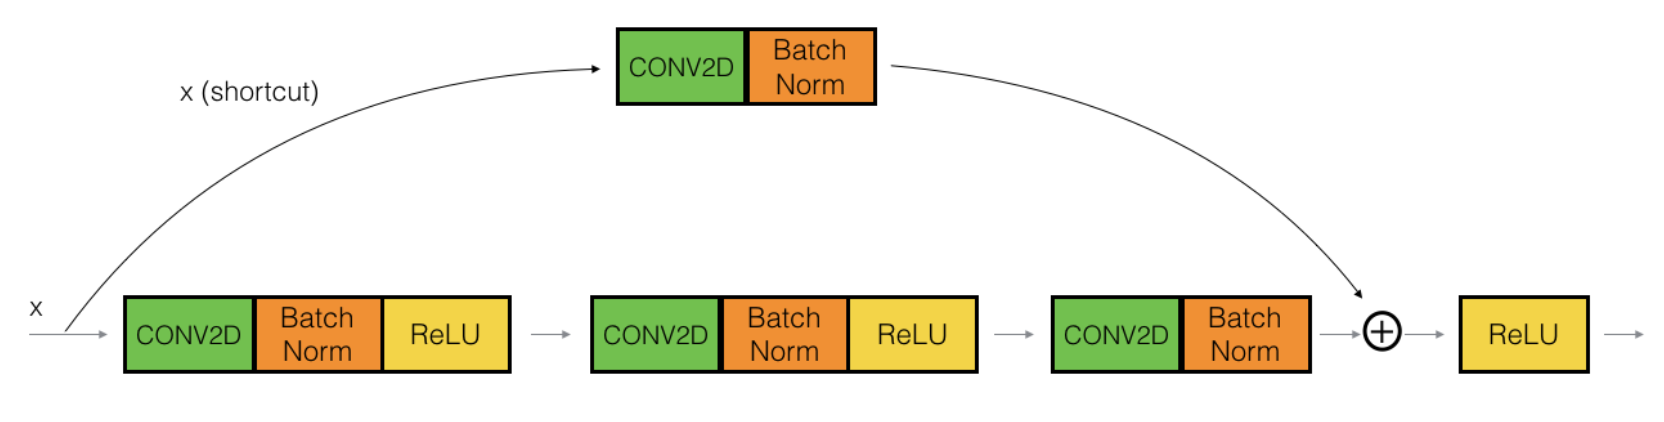
\includegraphics[width=\textwidth]{Figs/convolutionblock.png}
\caption{Convolutional Block \citep{resnet_implement}}
\label{convolutionblock}
\end{figure}

\item  Convolutional Block (Fig.\,\ref{convolutionblock}) is used when the input dimension does not match the output dimension. The only difference comparing to identity block is that convolutional block has a convolutional layer in the shortcut path to match the dimensions, formally defined in (\ref{eq2}).
    \begin{description}
      \item[$\ast$ First component of main path:] The first CONV2D has $F_1$ filters of shape (1,1) and a stride of $(s,s)$. Its padding is "valid". The first BatchNorm is normalizing the channels axis. Then apply the ReLU activation function. 
      \item[$\ast$ Second component of main path:] The second CONV2D has $F_2$ filters of shape $(f,f)$ and a stride of (1,1). Its padding is "same". The second BatchNorm is normalizing the channels axis. Then apply the ReLU activation function. 
      \item[$\ast$ Third component of main path:] The third CONV2D has $F_3$ filters of shape (1,1) and a stride of (1,1). Its padding is "valid". The third BatchNorm is normalizing the channels axis. There is no ReLU activation function.
      \item[$\ast$ Shortcut path:] The CONV2D has $F_3$ filters of shape (1,1) and a stride of $(s,s)$. Its padding is "valid". The BatchNorm is normalizing the channels axis. 
      \item[$\ast$ Final step:] The shortcut and the input are added together. Then apply the ReLU activation function.
    \end{description}
\end{enumerate}

The ResNet18 architecture is built as the following, modified from ResNet50 \citep{resnet50keras}:

\textbf{Stage 1}:
Zero-padding pads the input with a pad of (3, 3)
Convolution layer has 64 filters of shape (7, 7) and uses a stride of (2, 2).
BatchNorm is applied to the channels axis of the input.
MaxPooling uses a (3, 3) window and a (2, 2) stride.

\textbf{Stage 2}:
One convolutional block uses three set of filters $(F_1=F_2=F_3)$ of size [64, 64, 256], filter shape $f$ set to 3, stride $s$ set to 1.
Two identity blocks use three set of filters $(F_1=F_2=F_3)$ of size [64, 64, 256], filter shape $f$ set to 3.

\textbf{Stage 3}:
One convolutional block uses three set of filters of size [128, 128, 512], $f$ is 3, $s$ is 2.
Two identity blocks use three set of filters of size [64, 64, 256], $f$ is 3.

\textbf{Stage 4}:
One convolutional block uses three set of filters of size [256, 256, 1024], $f$ is 3, $s$ is 2.
Two identity blocks use three set of filters of size [256, 256, 1024], $f$ is 3.

\textbf{Stage 5}:
One convolutional block uses three set of filters of size  [512, 512, 2048], $f$ is 3, $s$ is 2.
Two identity blocks use three set of filters of size  [512, 512, 2048], $f$ is 3.

\textbf{Stage 6}:
One average pooling layer with a window of shape (2,2), followed by a flatten layer. Finally, a fully connected layer reduces its input to the number of classes using a softmax activation.
